\documentclass[9pt,letterpaper]{article}
\setlength{\textwidth}{16cm}
\setlength{\textheight}{22cm}
\hoffset-1.6cm
\voffset-2.4cm

%\usepackage{arxiv}
\usepackage[spanish]{babel}
\usepackage[utf8]{inputenc} % allow utf-8 input
%\usepackage[T1]{fontenc}    % use 8-bit T1 fonts
\usepackage{hyperref}       % hyperlinks
\usepackage{url}            % simple URL typesetting
%\usepackage{booktabs}       % professional-quality tables
\usepackage{amsfonts}
\usepackage{amsmath}
\usepackage{amssymb}       % blackboard math symbols
\usepackage{nicefrac}       % compact symbols for 1/2, etc.
\usepackage{microtype}      % microtypography
%\usepackage{lipsum}
\usepackage{graphicx}
%\usepackage{natbib}
\usepackage{multicol}
\usepackage{pgfkeys}
\usepackage{fancyhdr}
\usepackage{pstricks}
\usepackage{tcolorbox}
\tcbuselibrary{skins,breakable}   
\usepackage{tabularx}
\usepackage[shortlabels]{enumitem}
\usepackage{framed}
\usepackage{etoolbox}
\usepackage{tikz}
\usepackage{xparse}
\graphicspath{ {./Imagenes/} }
\usepackage[backend=bibtex]{biblatex}
\addbibresource{references.bib}


% Encabezados de página %%%%%
\pagestyle{fancy}
\headheight = 60pt
\fancyhead[L]{
	\parbox{3cm}{
		\begin{center}
			
\includegraphics[width=30pt]{Imagenes/ucentral.png}\\{\footnotesize \textbf{UNIVERSIDAD\\ CENTRAL}}
		\end{center}
	}
}
\fancyhead[R]{
	\parbox{13cm}{
		\begin{center}
			{\large \textsf{\textbf{FACULTAD DE INGENIERÍA Y CIENCIAS BÁSICAS}}}\\
			\textsf{\textbf{PREGRADO DE MATEMÁTICAS}}\\ 
			\textsf{\textbf{REGISTRO DE TRABAJO DE GRADO}}\\
			\textsf{\textbf{2021-I}}
		\end{center}
	}
}
%%%%%%%%%%%%%%%%%%%%%%%%%%%%%


%%  Ambientes institucionales del documento
%\newcounter{tcbcoro}[chapter]
%\renewcommand{\thetcbcoro}{\thechapter.\arabic{tcbcoro}}
\newtcolorbox{wwcoro}[2][]{%
	arc=0mm, % arc en las esquinas de las cajas
	breakable, % propiedad para la partición en variaspáginas
	enhanced,
	colback= white, % color del fondo de la caja
	boxrule=0.5pt, % ancho de la línea de la caja
	top=1mm,left=10pt, % delimitadores de texto interno
	fontupper={\small\bf\sffamily {#1}\;}~\normalfont,
	overlay unbroken  = { %barra vertical
		\draw[color=black,line width=1pt] ([xshift=0pt] frame.north west)--([xshift=0pt] frame.south west);               
	},%
	overlay first  = { %barra vertical
		\draw[color=black,line width=1pt] ([xshift=0pt] frame.north west)--([xshift=0pt] frame.south west);               
	},%
	% Mantener borde en cambio de página     
	overlay last ={\draw[color=black,line width=1pt] 
		([xshift=0pt] frame.north west)--([xshift=0pt] frame.south west);
	}     
	#1}


\newenvironment{estudiante}[5]{
	%begdef
\begin{sffamily}
	\begin{center}	
		\begin{tabular}{|c|c|l|c|l|c|l|p{6cm}|}\hline
			\multicolumn{7}{|l|}{NOMBRES: #1}& APELLIDOS: #2\\ 
			\hline
			TIPO DE IDENTIFICACIÓN:& T.I.&  &C.C.& \textbf{X} &C.E.& &NÚMERO: #3\\ \hline
			\multicolumn{7}{|l|}{CORREO INSTITUCIONAL: #4}& TELÉFONO: #5 \\
			\hline
		}{
		%enddef
		\end{tabular}
	\end{center}
\end{sffamily}
}

\newenvironment{docente}[4]{
	%begdef
	\begin{sffamily}
		\begin{center}	
			\begin{tabular}{|p{9cm}|p{6cm}|}\hline
				{NOMBRES: #1}& {DEPARTAMENTO: #2}\\ 
				\hline
				CORREO INSTITUCIONAL: #3& TELÉFONO-EXT: #4\\ \hline
			}{
				%enddef
			\end{tabular}
		\end{center}
	\end{sffamily}
}

\newenvironment{cajaseccion}[1]{
	\begin{center}
		\tcbox{ \textsf{\textbf{#1}} 
		}{
	}
	\end{center}
}

\newenvironment{fecha}[3]{
	\begin{flushright}\begin{tabular}{|c|c|c|c|}\hline
			\textsf{Fecha} & \textsf{#1} & \textsf{#2} & \textsf{#3}\\
			\hline
		}{	
		\end{tabular}
\end{flushright}
}

\newenvironment{titulo}[1]{
\begin{center}
	\begin{tabular}{|p{15.5cm}|}\hline
	\textsf{\textbf{1. TÍTULO DEL TRABAJO DE GRADO O PASANTIA:}} \\ \\
	#1 \\ }{ 	\hline
	\end{tabular}
\end{center}	
}

\newenvironment{introduccion}[1]{
\begin{center}
	\begin{tabular}{|p{15.5cm}|}\hline
	\textsf{\textbf{2. INTRODUCCIÓN Y JUSTIFICACIÓN (máximo 1500 palabras):}} \\
	#1 \\}{ \\ \hline
	\end{tabular}
\end{center}	
}

\newenvironment{introduccion2}[1]{
\begin{center}
	\begin{tabular}{|p{15.5cm}|}\hline
	\textsf{\textbf{}} }{ \\ \hline
	\end{tabular}
\end{center}	
}

\newenvironment{objetivo}{
	\begin{center}
		\begin{tabular}{|p{15.5cm}|}\hline
			\textsf{\textbf{3. OBJETIVO GENERAL:}} \\
			\\
		}{\\ \hline
		\end{tabular}
	\end{center}	
}

\newenvironment{especificos}{
	\begin{center}
		\begin{tabular}{|p{15.5cm}|}\hline
			\textsf{\textbf{4. OBJETIVOS ESPECÍFICOS:}}
		}{\\ \hline
		\end{tabular}
	\end{center}	
}

\newenvironment{antecedentes}[1]{
\begin{center}
	\begin{tabular}{|p{15.5cm}|}\hline
	\textsf{\textbf{5. ANTECEDENTES (máximo 2000 palabras):}} \\ \\
	#1 }{\\ \hline
	\end{tabular}
\end{center}	
}

\newenvironment{marcoTeorico}[1]{
\begin{center}
	\begin{tabular}{|p{15.5cm}|}\hline
	\textsf{\textbf{6. MARCO CONCEPTUAL:}}
	#1 }{\\ \hline
	\end{tabular}
\end{center}	
}

\newenvironment{metodologia}[1]{
\begin{center}
	\begin{tabular}{|p{15.5cm}|}\hline
	\textsf{\textbf{7. METODOLOGÍA:}} \\
	#1 \\}{ \\  \hline
	\end{tabular}
\end{center}	
}

\newenvironment{recursos}[1]{
\begin{center}
	\begin{tabular}{|p{15.5cm}|}\hline
	\textsf{\textbf{8. RECURSOS:}} \\
	#1 \\}{ \\  \hline
	\end{tabular}
\end{center}	
}

\newenvironment{cronograma}[1]{
\begin{center}
	\begin{tabular}{|p{15.5cm}|}\hline
	\textsf{\textbf{9. CRONOGRAMA DE ACTIVIDADES:}} \\
	#1 \\}{ \\  \hline
	\end{tabular}
\end{center}	
}


\newenvironment{esperados}{
	\begin{center}
		\begin{tabular}{|p{15.5cm}|}\hline
			\textsf{\textbf{11. RESULTADOS ESPERADOS: }} \\
			\\
		}{\\ \hline
		\end{tabular}
	\end{center}	
}

\newenvironment{presupuesto}{
	\begin{center}
		\begin{tabular}{|p{15.5cm}|}\hline
			\textsf{\textbf{10. PRESUPUESTO (En caso de modalidad Investigación) Y FUENTES DE FINANCIACIÓN (En caso de modalidad Profundización)}} \\
			\\
		}{\\ \hline
		\end{tabular}
	\end{center}	
}


\NewDocumentEnvironment{bibliografia}{O{} O{}}{\smallskip\begin{wwcoro}{#1}%
		\textsf{\textbf{10. BIBLIOGRAFÍA:}} \\
 		\begingroup
 		\renewcommand{\section}[2]{}
        \printbibliography
 		\endgroup
		{
	}\end{wwcoro}\smallskip }

\newenvironment{organizacion}[5]{
	\begin{center}
		\begin{tabular}{|p{4.5cm}|p{4.5cm}|p{5.5cm}|}\hline
			\multicolumn{3}{|l|}{\textsf{\textbf{13. DATOS DE LA ORGANIZACIÓN}(En caso de pasantía)}} \\ \hline
			\multicolumn{3}{|l|}{\textsf{NOMBRE DE LA ORGANIZACIÓN: #1}}\\ \hline
			\multicolumn{3}{|l|}{\textsf{RESPONSABLE DE LA ORGANIZACIÓN:#2}}\\ \hline
				\parbox{\linewidth}{\textsf{CORREO: \\#3}}&
			 	\parbox{\linewidth}{\textsf{TELÉFONO: \\ #4}} & 
			 	\parbox{\linewidth}{\textsf{DURACIÓN VINCULACIÓN (horas): \\ #5}}
		}{\\ \hline
		\end{tabular}
	\end{center}	
}

\newenvironment{firmas}{
\noindent	\textsf{\textbf{11. FIRMAS}}
	\begin{center} 
		\begin{tabular}{|p{7.5cm}|p{7.5cm}|}\hline
			\textsf{\textbf{FIRMA DEL ESTUDIANTE:}} &\textsf{\textbf{FIRMA DEL DIRECTOR O TUTOR:}} \\ \hline
			& \\
			& \\
			& \\
			& 
		}{\\ \hline
		\end{tabular}
	\end{center}	
}

\newenvironment{tramite}{
\noindent	\textsf{\textbf{12. DATOS DE TRÁMITE COMITÉ DE INVESTIGACIÓN DEL PROGRAMA} (Espacio para diligenciar por el Comité del Programa)}
	\begin{center}
		\begin{tabular}{|p{5cm}|p{5cm}|}\hline
			\textsf{\textbf{No.\n CONSECUTIVO}} & \\ 
			& \\ \hline
			\textsf{\textbf{No. ACTA}} & \\
			& \\ \hline
			\textsf{\textbf{FECHA}} & \\
			& 
		}{\\ \hline
		\end{tabular}
	\end{center}	
}




% % Corolario -------------------------------------------------------

%-

%%%%%%%%%%%%%%%%%%%%%%%%%%%%%%%%%%%%%%%%%%%%%5

%\title{}
%
%
%
%
%\author{
%Carlos Cortés \\
%  Dirección de estudiantes\\
%  Universidad Central\\
%  Bogotá, Colombia \\
%  \texttt{ccortesb@ucentral.edu.co} \\
%  \And
% David Peña \\
%  Maestría en analítica de datos\\
%  Universidad Central\\
%  Bogotá, Colombia \\
%  \texttt{dpenag2@ucentral.edu.co} \\
%  \And
%Diego Villada \\
%  Departamento de Matemáticas\\
%  Universidad Central\\
%  Bogotá, Colombia \\
%  \texttt{dvilladac1@ucentral.edu.co} \\
%}
%\maketitle
%\begin{abstract}
%El interés de las instituciones de educación superior en mantener el número de estudiantes matriculados ha llevado a diversos tipos de análisis estadísticos que soporten las campañas de permanencia. En este trabajo se busca encontrar y proponer una herramienta desde la analítica de datos que permita monitorear y controlar los factores de deserción más relevantes en el ámbito de la universidad central, a fin de identificar tempranamente a los estudiantes en condiciones propicias para la deserción.
%\end{abstract}


\begin{document}

\begin{center}
	\Large \textsf{\textbf{REGISTRO DE TRABAJO DE GRADO}}
\end{center}

\begin{fecha}{31}{05}{2021} \end{fecha}

\begin{cajaseccion}{DATOS DEL ESTUDIANTE }\end{cajaseccion}


\begin{estudiante}{JORGE ANDRES}{IBAÑEZ HUERTAS}{1001045370}{jibanezh@ucentral.edu.co}{3045560527}
\end{estudiante}


% keywords can be removed
%\keywords{Deserción académica, Analítica de datos, métodos estadísticos multivariados, machine learning, tableros de control}

% \begin{cajaseccion}{MODALIDAD DE TRABAJO DE GRADO (Seleccione una opción) }\end{cajaseccion}


% \begin{center}
% 	\begin{tabular}{|p{7cm}|p{7cm}|}\hline
% 		\textbf{I. Modalidad de investigación} & \textbf{II. Modalidad de profundización:}\\
% 		\hline
% 		\parbox{6.8cm}{a. Proyecto final con resultados de nuevo conocimiento:( )  }
% 		&\parbox{6.8cm}{a. Trabajo monográfico: (X)  }\\
% 		\hline
% 		&\parbox{6.8cm}{b. Pasantía nacional o internacional: ( )   }\\
% 		\hline
% 	\end{tabular}
% \end{center}

% \begin{center}
% 	\begin{tabular}{|p{14cm}|} \hline
% 		\textbf{Línea de profundización} \\ 
% 		\hline
% 		% Escriba acá la línea de profundización si aplica        
% 		\\
% 		\hline
% 	\end{tabular}
% \end{center}

\begin{cajaseccion}{AVAL DEL DOCENTE DIRECTOR}\end{cajaseccion}

\begin{docente}{
		CARLOS ISAAC ZAINEA}{
		MATEMÁTICAS}{
		czaineam@ucentral.edu.co}{
		3239868 - 3457}
\end{docente}

\begin{cajaseccion}{COMPONENTES}
\end{cajaseccion}

\begin{titulo}{Diseño de un algoritmo en redes neuronales para predecir el comportamiento de una enfermedad, en entornos simulados con autómatas celulares}
\end{titulo}


\begin{introduccion}{}
	Las matemáticas han sido pieza fundamental en el estudio epidemiológico, el cual busca predecir el comportamiento de una enfermedad para mitigar su impacto, tomando medidas de control y prevención. 

Un punto de partida es el modelo descrito por Kermack y McKendrick en 1927, también conocido como modelo SIR, en el que se establecen relaciones entre tres estados de una enfermedad (Susceptible-Infectado-Recuperado) y se implementan los conceptos de tasa de contagio y de recuperación \cite{malariaSIR}. Desde entonces se han desarrollado múltiples variaciones sobre el modelo SIR, con el objetivo de analizar diferentes tipos de enfermedades de una manera más precisa, considerando por ejemplo diferentes estados, tasas de natalidad y mortalidad, entre otros \cite{diego2010}.

Por otra parte y debido a los avances tecnológicos de las últimas décadas, se han desarrollado modelos y simulaciones que permiten analizar características que no eran posibles con los modelos anteriormente mencionados. Por ejemplo, patrones de movilidad \cite{colaGNN, epidemiologicalNeuralNetwork}, disminución en la cantidad de contagios debido a un aislamiento preventivo \cite{stayHome}, contagios de individuo a individuo \cite{heterogeneousPopulation} e interacciones en masa \cite{combiningGraph, transfer2021}, la mayoría realizadas con una fuerte influencia de las redes neuronales y complejas, apoyadas fuertemente sobre la teoría de grafos. 

La inexistencia de un algoritmo predictivo que tenga en cuenta las interacciones más cercadas de cada individuo, es un problema que se ha evidenciado principalmente, a causa de la naturaleza de las bases de datos disponibles. A pesar del fuerte acercamiento de los modelos epidemiológicos a las dinámicas sociales con la llegada del coronavirus, se consideran interacciones a escalas que podrían ser mayores a las que se contagia la enfermedad, si bien existen modelos que analizan dinámicas de persona a persona, sus capacidades predictivas resultan limitadas por la naturaleza con la que se generan las bases de datos, como ocurre en \cite{combiningGraph,transfer2021}.

Teniendo en cuenta la aplicabilidad de los autómatas celulares y las cualidades predictivas de los modelos en redes neuronales, se pretende simular el comportamiento de una enfermedad y desarrollar un algoritmo que permita realizar pronósticos sobre su comportamiento, para responder a la pregunta: ¿Qué impacto tienen las relaciones sociales cercanas, en la propagación de una enfermedad?
\end{introduccion}

\begin{introduccion2}{}
    Este trabajo permitirá comprender de manera más certera, como las interacciones de las personas afectan la propagación de alguna enfermedad y podrá establecer características para construir las bases de datos, que pueden dar lugar a análisis predictivos más realistas. Así mismo, se abre la puerta a que se propongan diferentes algoritmos con el fin de obtener diferentes resultados óptimos que alimenten el estudio epidemiológico. 
\end{introduccion2}

\begin{objetivo}
	\input{03-objetivos}
\end{objetivo}

\begin{especificos}
	%Objetivos específicos

\begin{enumerate}
    \item Comprender las dinámicas descritas por los modelos SIS y SIR.
	\item Diseñar e implementar un modelo matemático para describir y simular la propagación de una enfermedad por medio de un algoritmo basado en autómatas celulares.
	\item Interpretar las curvas descritas por el modelo en autómatas celulares y realizar una comparación con los modelos compartiméntales clásicos.
	\item Desarrollar herramientas que permitan analizar el comportamiento de la enfermedad, considerando diferentes topologías para los autómatas.
    \item Diseñar e implementar un algoritmo en redes neuronales que permita realizar pronósticos sobre el comportamiento de la enfermedad simulada.
    \item Definir métricas que permitan establecer la eficiencia del algoritmo propuesto en redes neuronales frente a cambios de topología en el modelo en autómatas celulares.
\end{enumerate}
\end{especificos}

\begin{antecedentes}{}
	\input{05-antecedentes}
\end{antecedentes}

\begin{introduccion2}{}
    Otra aplicación interesante es el modelo desarrollado en \cite{colaGNN}, el cual se centra en la predicción de los ILI a largo plazo, usando datos con un rango de tiempo limitado a 20 semanas. Teniendo presente la perdida de información temporal, exploran un modelo de propagación en grafos con representaciones espaciales. Usan además, las redes neuronales recurrentes para capturar las dependencias secuenciales en los datos de las series temporales locales y diseñan un módulo de convolución temporal para extraer automáticamente las dependencias temporales cortas y largas de los datos de series temporales de múltiples localizaciones.

Encontramos también aplicaciones entre la teoría de redes y la epidemiología. Moo Kim realiza un análisis interesante para la propagación de enfermedades en redes complejas, puntualmente en la red de Barabasi-Albert, presente en diversas redes reales \cite{redesComplejas}. Realiza además, una implementación de los modelos compartiméntales clásicos en redes regulares y complejas.

Desplazándonos un poco a la teoría de redes neuronales y los procesos de machine-learning, encontramos trabajos como el de Schmidt en \cite{schmidt2019}, en donde implementa una red neuronal artificial, basada en modelos compartiméntales para predecir la propagación del virus de la influenza, para posteriormente realizar una comparación con un modelo de regresión lineal múltiple.

La reciente aparición del coronavirus a finales del 2019, ha incentivado estudios que proponen diversos enfoques basados en redes neuronales convolucionales de grafos (GCNs), memorias de corto plazo (LSTMs) y modelos de aprendizaje de transferencia basados en el meta-aprendizaje (MAML) \cite{combiningGraph, epidemiologicalNeuralNetwork}. Mientras que en \cite{epidemiologicalNeuralNetwork} proponen un modelo basado en machine-learning para estimar los parámetros de un modelo epidemiológico que se ajusta a tendencias observadas sobre el movimiento de individuos, en \cite{combiningGraph} proponen un enfoque de fusión entre redes neuronales basadas en grafos y modelos epidemiológicos para combinar directamente los datos de movilidad diádica y conectividad derivadas de Facebook con información estructural y espacial de distritos alemanes.

Panagopoulos, Nikolentzos y Michalis Vazirgiannis realizan un trabajo comparable en \cite{transfer2021}, en donde se centran en predecir el comportamiento de la enfermedad basándose en los datos de movilidad de masa, y consideran la circulación dentro de una región como un indicador de interacción. Exponen además, la inexistencia de una base de datos que considere las posibles interacciones entre individuos y sus implicaciones.

Después de revisar diferentes desarrollos en el campo de la epidemiología, se ratifica la importancia de un análisis predictivo que tenga en cuenta las relaciones o interacciones más cercanas, de modo que se establezcan estrategias de prevención y contención mucho más certeras.

\end{introduccion2}

\begin{marcoTeorico}{}
\section*{Modelos compartimentales}
Los modelos compartiméntales reciben su nombre por ser modelos en los que la población se divide en ''compartimientos'', de modo que cada individuo solo pueda pertenecer a una de las divisiones y asumiendo además, que todos los individuos en un mismo compartimiento tengan exactamente las mismas características.

\subsection*{El modelo SIS}

El modelo $SIS$ describe la interacción entre dos estados, susceptible (S) e infectado (I), el paso de un estado a otro viene determinado por las constantes $\alpha$ y $\beta$, las cuales representan las tasas de recuperación e infección respectivamente.


\end{marcoTeorico}

\begin{introduccion2}{}
    \begin{center}
	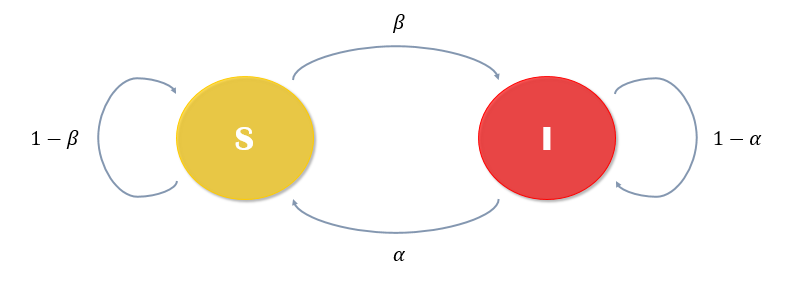
\includegraphics[width=0.65\linewidth]{Imagenes/esquema_sis.PNG}
\end{center}

\begin{center}
    \caption{Fuente: Jorge Ibañez 2021} \\
\end{center}

De donde se obtiene el siguiente sistema de ecuaciones diferenciales:
\begin{equation}
    \left\{
    \begin{array}{c}
        S' = \alpha I - \beta SI \\
        I' = \beta SI - \alpha I
    \end{array}
    \right. \label{eq:1}
\end{equation}

Para modelar el comportamiento de los individuos mediante el sistema de ecuaciones diferenciales descrito en \ref{eq:1}, se consideran los contactos entre las poblaciones de susceptibles e infectados a partir del producto de las variables S e I. 

El término $\alpha I$ indica la probabilidad de que un individuo se recupere mientras que el término $\beta SI$ indica la probabilidad de que un individuo susceptible se infecte al de tener contacto con un individuo infectado. \cite{diego2010}

\subsection*{El modelo SIR}

A diferencia del modelo SIS, el modelo SIR describe las interacciones entre los estados susceptible (S), infectado (I) y recuperado (R). Es posible que un individuo susceptible adquiera el virus y que posteriormente pueda recuperarse, sin embargo en este modelo no es posible que un individuo que no ha tenido la enfermedad en algún momento se cure de esta, para comprender de una mejor manera el funcionamiento del modelo $SIR$ observemos el siguiente diagrama:

\begin{center}
	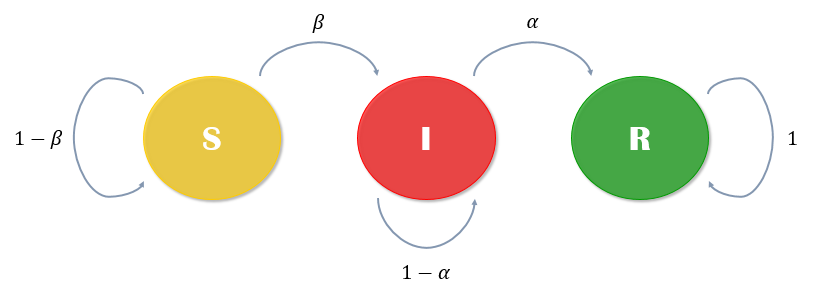
\includegraphics[width=0.7\textwidth]{Imagenes/esquema_sir.PNG}
\end{center}
\begin{center}
    \caption{Fuente: Jorge Ibañez 2021}
\end{center}

Al igual que en el caso del modelo $SIS$, las constantes $\alpha$ y $\beta$ representan las tasas de recuperación e infección respectivamente; una vez dicho esto podemos describir el modelo $SIR$ en ecuaciones diferenciales:
\begin{equation}
    \left\{
    \begin{array}{l}
        S' = -\beta SI \\
        I' = \beta SI-\alpha I \\
        R' = \alpha I
    \end{array}
    \right.\label{equ3}
\end{equation}

\end{introduccion2}

\begin{introduccion2}{}
    Tal y como ocurría en el modelo SIS, los contactos entre poblaciones se van a representar con el producto de variables y los factores $\alpha I$ y $\beta SI$ serán equivalentes respectivamente, a la recuperación de un porcentaje $\alpha$ de individuos infectados y al paso al estado de infección por parte de un porcentaje $\beta$ de individuos susceptibles, luego de tener contacto con infectados\cite{diego2010}.

\section*{Autómatas celulares}
Son un modelo matemático capaz de describir el comportamiento de diferentes sistemas dinámicos, están compuestos por un conjunto de agentes (también llamados celdas, células, individuos o píxeles) que toman algún valor o estado.

El \textit{estado} de cada individuo es alterado en mediciones discretas de tiempo, usualmente esta alteración del estado de la célula depende del comportamiento sus individuos cercanos también llamados \textit{vecinos}, la regla que describe la relación entre el conjunto de estados, el agente y sus vecinos está determinada por una expresión matemática la cual se conoce la \textit{regla de evolución local}.\cite{descripcionyAplicaciones}

Para definir las reglas de evolución local de manera que se tengan en cuenta las tasas de infección y de recuperación, junto con el estado de cada vecino se usarán las reglas semi-totalísticas, las cuales consideran el estado de la célula central para posteriormente asignar un elemento del conjunto de estados a la suma de los valores de los elementos que forman la vecindad, estos valores determinan el comportamiento de todas las vecindades cuya suma de valores de sus elementos corresponda a un mismo valor.\cite{ACaplicacionesComputacion}

Cada individuo puede tomar un único valor del conjunto de estados que se modelan con el autómata celular, en nuestro caso será uno de dos estados para el modelo SIS (o tres en el caso del modelo SIR). Es importante resaltar la complejidad que puede llegar a tener un autómata celular, debido al comportamiento en la vecindad de cada celda.

En el caso de sistemas 2-dimensionales encontramos una gran cantidad de vecindades, entre las más conocidas encontramos la \textit{vecindad de Von Neumann} la cual considera a la célula central y a los individuos ubicados a la izquierda, derecha, arriba y abajo y la \textit{vecindad de Moore} la cual añade los individuos diagonales a la vecindad de Von Neumann. Para los intereses del proyecto, se decidió trabajar con vecindades de Moore. 

\begin{center}
	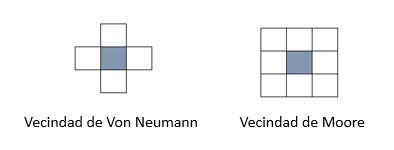
\includegraphics[width=0.5\textwidth]{Imagenes/vecindades.PNG}
\end{center}
\begin{center}
    \caption{Fuente: Jorge Ibañez 2021}
\end{center}

Aunque si bien, la investigación iniciará sobre las redes regulares definidas sobre las vecindades de Von Neumann y las vecindades de Moore, lo ideal es implementar diferentes tipos de vecindad que permitan fortalecer los aspectos predictivos del algoritmo en redes neuronales. Para esto será necesario tener presentes algunas nociones de topologías definidas a partir de vecindades.

\section*{Topología}
Durante esta sección se mencionan algunos de los conceptos relacionados con topología que se usaran durante el desarrollo del proyecto. Uno de los objetivos del proyecto es analizar el impacto de los cambios de topología, para lo cual debemos tener presentes los conceptos de topología definida por un sistema de vecindades, familias de vecindades entre otros. Se desarrolló una recopilación de definiciones extraídas de \cite{filtrosTopologia,munkres,elementosTopologiaGeneral}.
\end{introduccion2}

\begin{introduccion2}{}
    \textbf{Definición (Topología):} Para $X$ un conjunto no vacío y $\tau$ una colección de subconjuntos dé $X$. Conoceremos a $\tau$ como una \textit{topología} sobre $X$ si:

\begin{enumerate}
    \item $\emptyset$ y $X$ están en $\tau$.
    \item La unión de elementos de cualquier sub colección de $\tau$ es un elemento en $\tau$.
    \item Toda intersección finita de elementos de $\tau$ esta en $\tau$.
\end{enumerate}

Diremos que la dupla $(X,\tau)$ es un \textit{espacio topológico} si $\tau$ es una topología sobre $X$, adicionalmente conoceremos a los elementos de $\tau$ como \textit{conjuntos abiertos}. 

\textbf{Definición (Subespacio):} Para $Y$ un subconjunto del espacio topológico $X$, la colección $\tau'=\{A\cap Y|A\in \tau\}$ es una \textit{topología sobre} $Y$, la cual conoceremos como \textit{topología relativa de} $Y$. Con esta topología, $Y$ se denomina \textit{subespacio} de $X$.

\textbf{Definición (Vecindades):} Consideremos ahora un elemento $x$ en el espacio topológico $X$, diremos que un conjunto $V$ es una \textit{vecindad de} $x$ si existe $A\in\tau$ tal que $x\in A\subset V\subset X$. A la \textit{familia de vecindades} de $x$ las denotaremos como $\mathcal{V}(x)$. 

\textbf{Proposición:} Para la familia de vecindades de $x$ se cumplen las siguientes propiedades:

\begin{enumerate}
    \item Si $U\in\mathcal{V}(x)$, entonces $x\in U$.
    \item Si $U,V\in\mathcal{V}(x)$, entonces $U\cap V\in\mathcal{V}(x)$.
    \item Si $U\in\mathcal{V}(x)$ y $u\subset V\subset X$, entonces $V\in\mathcal{V}(x)$.
    \item Para cada $U\in\mathcal{V}(x)$ existe $V\in\mathcal{V}(x)$ tal que $U\in\mathcal{V}(y)$ para cada $y\in V$.
\end{enumerate}

% \textit{Demostración:} Claramente $(1)$ se deduce de la definición 1.3. Para mostrar $(2)$, note que como $U\in\mathcal{V}(x)$, existe $A\in\tau$ tal que $x\in A\subset U$, de manera similar existe $B\in\tau$ tal que $x\in B\subset V$. De ese modo tenemos que $x\in A\cap B\subset U\cap V$, donde en particular $A\cap B\in\tau$, concluimos con esto que $U\cap V\in\mathcal{V}(x)$.

% Dado que $U\in\mathcal{V}(x)$ existe $A\in\tau$ tal que $x\in A\subset U$, como por hipótesis tenemos $U\subset V$, en particular $x\in A\subset V$ con $A\in\tau$, con lo cual hemos mostrado $(3)$.

% Para el caso de $(4)$, considere $U\in\mathcal{V}(x)$ arbitrario, luego por la definición 1.3 existe $V\in\tau$ tal que $x\in V\subset U$, con lo cual $V\in\mathcal{V}(x)$. De ese modo, para todo $y\in V$ se tiene que  $y\in V\subset U$ donde $V\in\tau$, se sigue que $U\in\mathcal{V}(y)$ para $y\in V$.

% $\hfill\square$

\textbf{Definición (Base de una topología):} Definimos la \textit{base} $\mathcal{B}$ de la topología de un conjunto $X$, como la colección de subconjuntos de $X$ tales que:
\begin{enumerate}
    \item Para cada $x\in X$, existe por lo menos un elemento $B\in\mathcal{B}$ que contiene a $x$.
    \item Sí $x\in B_1\cap B_2$, para $B_1,B_2\in\mathcal{B}$, entonces existe $B_3\in\mathcal{B}$ tal que $x\in B_3$ y $B_3\subset B_1\cap B_2$.
\end{enumerate}

\textbf{Definición (Abierto):} Para $\mathcal{B}$ una base de una topología sobre $X$, un subconjunto $U$ de $X$ se dice que es \textit{abierto} de $X$, si para cada $x\in U$, existe $B\in\mathcal{B}$ tal que $x\in B$ y $B\subset U$. La colección de subconjuntos $U$ con esta propiedad, se define topología generada por $\mathcal{B}$.

\textbf{Definición (Base de vecindades):} Diremos que una colección $\mathcal{B}(x)\subset\mathcal{V}(x)$ es una \textit{base de vecindades de $x$} en el espacio topológico $(X,\tau)$, con $x\in X$, sí para cada $V\in\mathcal{V}(x)$ existe $B\in\mathcal{B}(x)$ tal que $B\subset V$.

\textbf{Proposición:} Sea $(X,\tau)$ un espacio topológico, supongamos que para cada $x\in X$ hemos elegido una base de vecindades $\mathcal{B}(x)$, entonces
\begin{enumerate}
    \item Si $V_1,V_2\in\mathcal{B}(x)$, entonces existe $V_3\in\mathcal{B}(x)$ tal que $V_3\subset V_1\cap V_2$.
    \item Para cada $V\in\mathcal{B}(x)$ se puede escoger $V_0\in\mathcal{B}(x)$ de modo que para $y\in V_0$, existe $W\in\mathcal{B}(y)$ tal que $W\subset V$.
\end{enumerate}

% \textit{Demostración:} Para mostrar $(1)$ tome $V_1, V_2\in\mathcal{B}(x)$, donde por definición sabemos que existen abiertos $A_1$ y $A_2$ tales que $x\in A_1\subset V_1$ y $x\in A_2\subset V_2$, con lo cual $x\in A_1\cap A_2\subset V_1\cap V_2$ y $A_1\cap A_2\in\mathcal{V}(x)$. Dado que $\mathcal{B}(x)$ es una base de vecindades, existe $V_3\in\mathcal{B}(x)$ tal que $x\in V_3\subset A_1\cap A_2\subset V_1\cap V_2$.

% Por otra parte, para mostrar $(2)$ observe que en particular $V\in\mathcal{V}(x)$, con lo cual podemos afirmar que existe $A\in\tau$ tal que $x\in A\subset V$. Dado que $\mathcal{B}(x)$ es una base de vecindades, existe $V_0\in\mathcal{B}(x)$ tal que $x\in V_0\subset A$.

% Note que para todo $y\in V_0$, tenemos que $y\in A$ y con lo cual $A\in\mathcal{V}(y)$, si escogemos una base de vecindades de $y$, digamos $\mathcal{B}(y)$, tenemos que existir $W\in\mathcal{B}(y)$ tal que $y\in W\subset A\subset V$, concluyendo así la prueba. 

% $\hfill\square$

\textbf{Definición (Frontera de un conjunto):} Definimos la \textit{frontera} de un conjunto $A\subset X$, como el conjunto de puntos $x\in X$ tales que para todo $V\in\mathcal{V}(x)$ se cumple que $V\cap A\neq\emptyset$ y $V\cap(X\setminus A)\neq\emptyset$.

\end{introduccion2}

\begin{metodologia}{}
	\input{07-metodologias}
\end{metodologia}

\begin{introduccion2}{}
    \input{07-metodologias1}
\end{introduccion2}

\begin{introduccion2}{}
    Posteriormente se realizarán las modificaciones sobre la topología con la que se simuló la enfermedad en la primera fase. Para esto, será necesario implementar una herramienta que permita definir y modificar la topología sobre la cual se desarrollan las simulaciones.

Una vez se realice dicha implementación, se desarrollarán las validaciones finales sobre el algoritmo en redes neuronales, con lo que se espera poner a prueba la efectividad del algoritmo propuesto.
\end{introduccion2}

\begin{recursos}{}
	% Recursos

Se espera que el proyecto este desarrollado en su totalidad sobre Python 3.8.

Puntualmente para el desarrollo de la simulación, se usarán las librerías \textbf{numpy} para cálculos sobre arreglos matriciales; \textbf{matplotlib, cv2 y seaborn} para visualizaciones y algunas características; \textbf{random y scipy.stats} para valores aleatorios. Mientras que el desarrollo del algoritmo en redes neuronales se usarán las librerías \textbf{Keras, TensorFlow y PyTorch}.
\end{recursos}

\begin{cronograma}{}
	%\section{Cronograma}

Los tiempos estimados para la ejecución del proyecto se presentan en la siguiente tabla:

\begin{center}
	\includegraphics[width=1\linewidth]{Imagenes/Cronograma}
\end{center}

\end{cronograma}

% \begin{presupuesto}
% 	% Presupuesto

Para la realización del proyecto se ha presupuestado que solo serán necesarios los computadores de los autores para poder realizar cálculos de modelos y refinamiento de la data. De ser necesario, se recurirá a un servicio en nube para el almacenamiento de los datos y una máquina virtual, también en nube, para mantener el tablero corriendo. 
% \end{presupuesto}

% \begin{esperados}
% 	% Resultados esperados

La finalidad del tablero de control es monitorear las variables que apalancan la desición de retiro de los estudiantes de la universidad, así que se busca dicho tablero logre dar tanto a los directivos como a los responsables de la emisión de alertas tempranas una herramienta para la identificación de los posibles casos de abandono.
% \end{esperados}

\begin{bibliografia}
% \printbibliography
\end{bibliografia}

\begin{firmas}
\end{firmas}

\begin{tramite}
\end{tramite}

\end{document}
